%%
%% This is file `esapub.tex',
%% generated with the docstrip utility.
%%
%% The original source files were:
%%
%% esapub.dtx  (with options: `manual')
%% ============================================
%% This is the manual describing the usage of
%%      esapub.cls
%% ============================================
%% Copyright 1999 Patrick W Daly
%% Max-Planck-Institut f\"ur Aeronomie
%% Max-Planck-Str. 2
%% D-37191 Katlenburg-Lindau
%% Germany
%% E-mail: daly@linmpi.mpg.de
%%
%% -------------------------------------------------
\ProvidesFile{esapub.tex}
          [2001/04/25 1.1 (PWD)]
\documentclass[a4paper,twocolumn]{esapub2005} % European paper
\pagestyle{empty}

% introduce this option for the ESA publications style
\bibliographystyle{alpha}

\usepackage{times}
\usepackage{natbib}
\usepackage{graphicx}

\title{Aspects of the RPW antennas of SOLAR ORBITER}
\author[*]{Oswald T.H.}
\author[*]{H.O. Rucker}
\author[*]{W. Macher}
\affil[*]{Space Research Institute, Austrian Academy of Sciences, A-8042 Graz, Austria, thomas.oswald@oeaw.ac.at}
\author[ ]{the SOLAR ORBITER RPW team}

\newcommand{\btx}{\textsc{Bib}\TeX}
\newcommand{\filename}{esapub}

\begin{document}

\keywords{SOLAR ORBITER, STEREO, radio science, antenna calibration}

\maketitle

\begin{abstract}
SOLAR ORBITER is a very ambitious spacecraft mission which constitutes the next generation of solar exploration. On board is, besides several other experiments, the radio plasma and waves analyzer (RPW) which will be designed to receive electrostatic as well as electromagnetic waves, therefore enabling in-situ as well as remote sensing measurements. The RPW experiment is very similar to the SWAVES experiment on the STEREO spacecraft. In this paper we use our experience with the SWAVES antennas to discuss several aspects of the scientific antennas which will be mounted on SOLAR ORBITER.
\end{abstract}

\section{Introduction}
The radio plasma and waves analyzer (RPW) of SOLAR ORBITER will be designed to receive electrostatic as well as electromagnetic waves, therefore enabling in-situ as well as remote sensing measurements. The Plasma Waves Analyser (PWA) will cover the in-situ measurements while the Radio Spectrum Analyzer (RAS) will be responsible for the remote sensing. Both subsystems will share the same sensors, especially the electric field antennas (RPW-antennas).

Quasi-thermal Noise Spectroscopy and Direction Finding, i.e. the technique to determine the direction of incidence and the state of polarization from the measured data, will play an important part in the science done in the course of this mission. Certain requirements have to be fulfilled such that these techniques can be successfully applied.

The RPW experiment is very similar to the SWAVES experiment on the STEREO spacecraft. In this paper we use our experience with the SWAVES antennas to discuss the mentioned requirements and limitations to be expected on SOLAR ORBITER.

\section{Solar Orbiter}
The Solar Orbiter mission will provide the next major step forward in the exploration of the Sun and the heliosphere to solve many of the fundamental problems remaining in solar and heliospheric science. It incorporates both a near-Sun and a high-latitude phase. The near-Sun phase of the mission enables the Orbiter spacecraft to approach the Sun as close as 48 solar radii (~0.22 AU) during part of its orbit, thereby permitting observations from a quasi-heliosynchronous vantage point (so-called co-rotation).


The main objectives are :

\begin{itemize}
    \item Determine the properties, dynamics and interactions of plasma, fields and particles in the near-Sun heliosphere.
    \item Investigate the links between the solar surface, corona and inner heliosphere.
    \item Explore the energetics, dynamics and fine-scale structure of the magnetized atmosphere at all latitudes.
    \item Probe the solar dynamo by observing the Sun's high-latitude field, flows and seismic waves.
\end{itemize}


Figures \ref{fig:antennas1} and \ref{fig:antennas2} show the two different antenna configurations which could be used for SOLAR ORBITER. The design consisting of 3 antennas shown in Figure \ref{fig:antennas1} is very similar to the configuration used for the SWAVES experiment (see Figure \ref{fig:wiregrid}). The second possible design comprises 4 antennas which are set up in a way to give a very good nearly isotropic power pattern. It is similar to the system used for the RESONANCE mission (see Figure \ref{fig:resonance}).

It can be expected that the effective length vectors of configuration in Figure \ref{fig:antennas1} would behave similar to the behavior of the electric antennas of the STEREO mission. The order of magnitude of the length of the effective length vectors of configuration in Figure \ref{fig:antennas2} will also be similar to STEREO, while the directions will deviate considerably due to the different influence of the spacecraft hull.

\begin{figure}
\centering
  \includegraphics[width=1.0\linewidth]{paperpics/antennas1.eps}
\caption{A possible antenna configuration for SOLAR ORBITER.\label{fig:antennas1}}
\end{figure}

\begin{figure}
\centering
  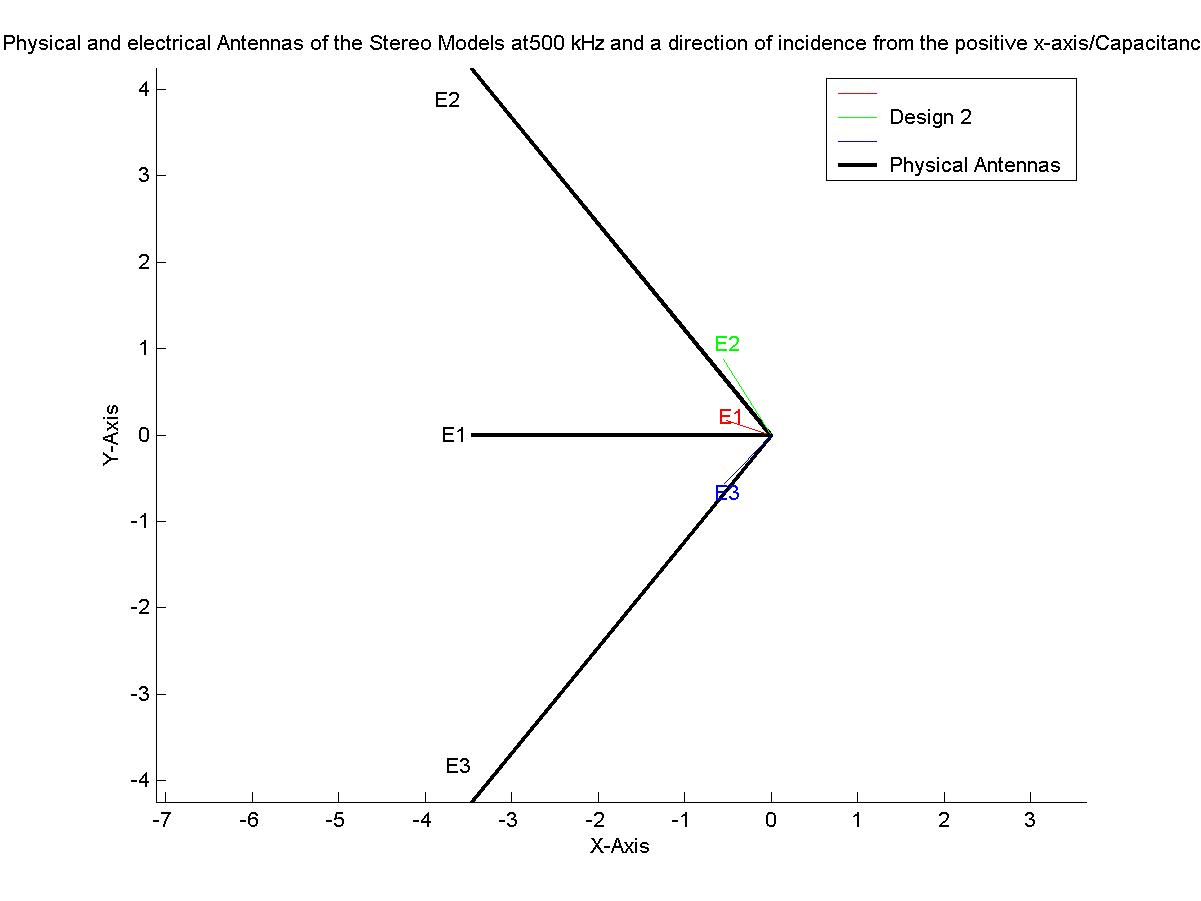
\includegraphics[width=1.0\linewidth]{paperpics/antennas2.eps}
\caption{Another possible antenna configuration for SOLAR ORBITER.\label{fig:antennas2}}
\end{figure}

\begin{figure}
\centering
  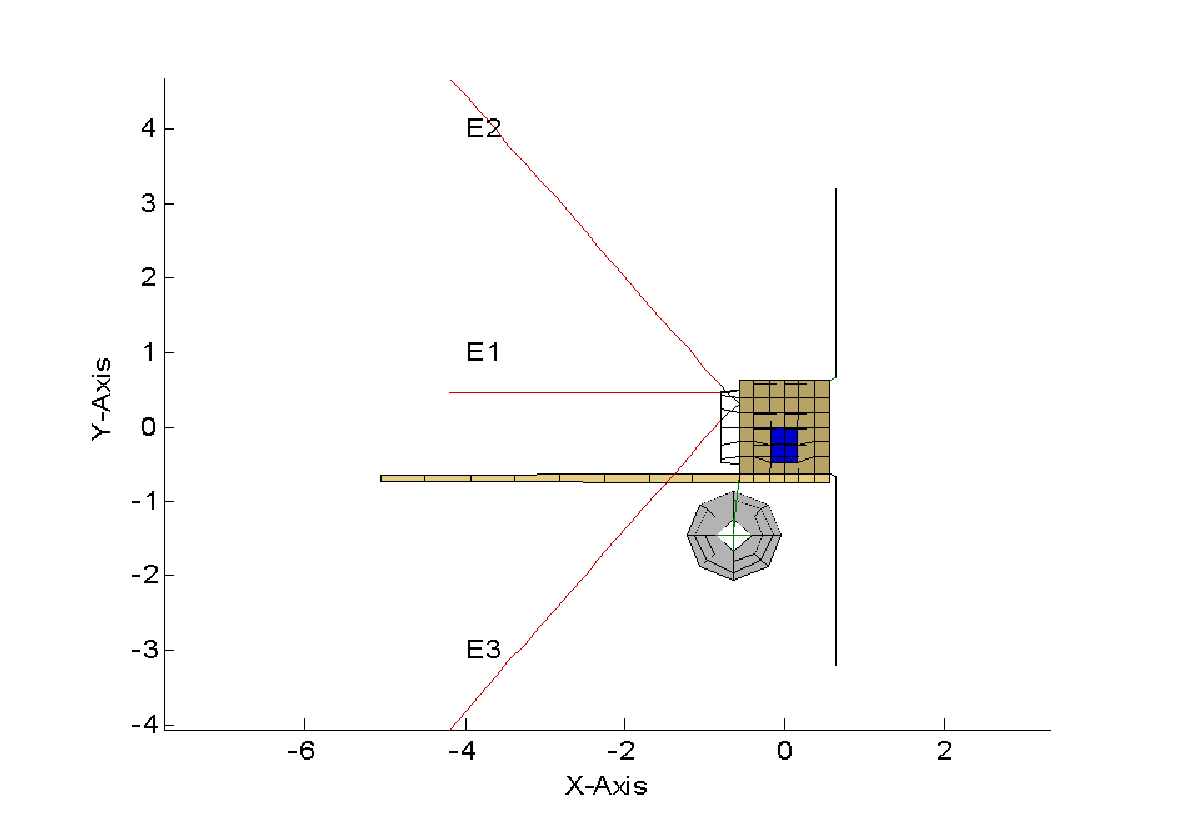
\includegraphics[width=1.0\linewidth]{paperpics/stero_wiregrid.eps}
\caption{Wire-grid model of the STEREO spacecraft.\label{fig:wiregrid}}
\end{figure}

\begin{figure}
\centering
  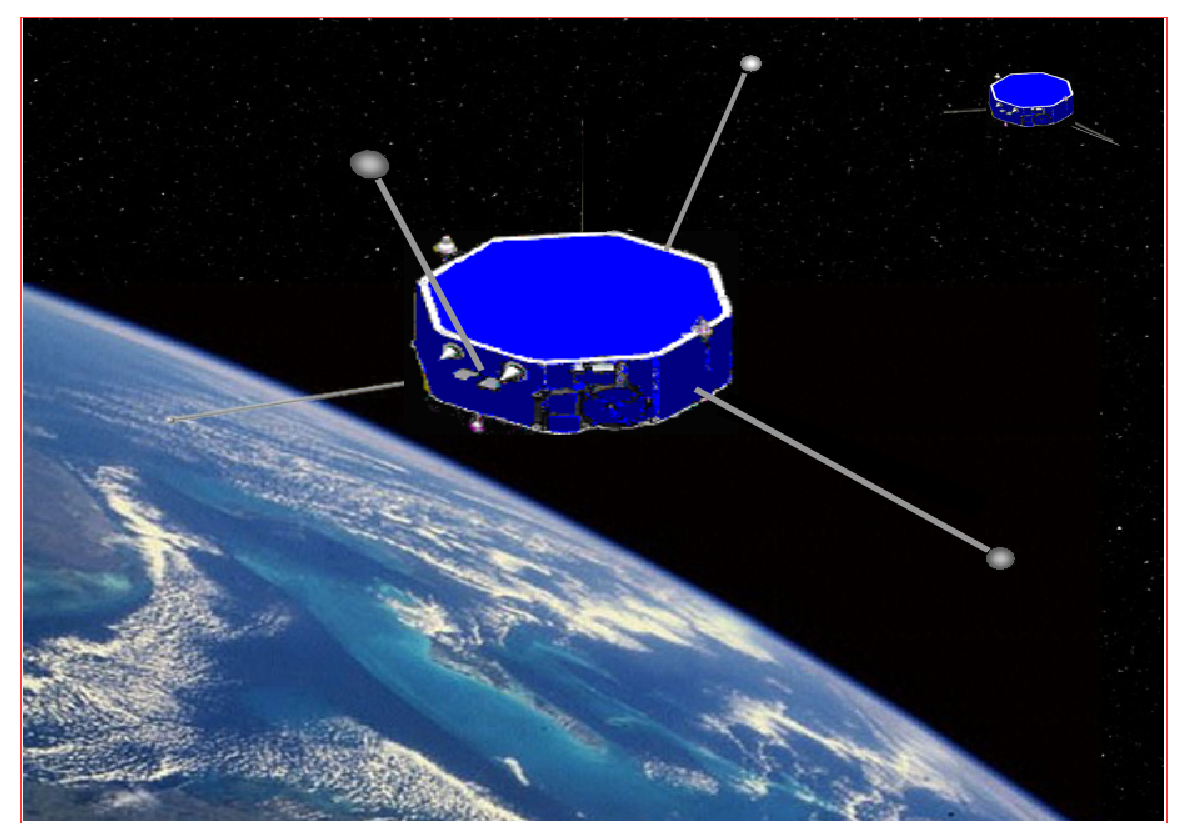
\includegraphics[width=1.0\linewidth]{paperpics/resonance.eps}
\caption{Artist's view of the RESONANCE spacecraft.\label{fig:resonance}}
\end{figure}

\section{Calibration of spacecraft antennas}
For the correct interpretation of the produced data it is of vital importance to know the antenna properties with great accuracy. Because of the fact that the skin of the spacecraft is made of conducting material, it is electromagnetically coupled to the monopoles and has, therefore, to be considered as part of the antenna system. As a result the properties of the antennas depend to a great extent on the geometric shape of the spacecraft hull, which makes it hard to determine their behavior. Additionally the surrounding space plasma can have an appreciable influence on the antenna properties. Several methods have been developed to calibrate spacecraft antennas:

\begin{itemize}
    \item Numerical wire-grid modeling
\item Experimental rheometry
\item Experimental anechoic chamber
\item In-flight calibration
\end{itemize}

For the numerical method the spacecraft is modeled by short wire segments. Instead of the surface currents which are induced as response to the incident radiation, only currents along these wire segments are dealt with. As long as the mesh size is smaller than the wavelength, this method shows good results. The currents are calculated by use of the method of moments, a widely used technique working in the frequency domain \cite{harrington}. On base of the currents all other antenna properties of interest can be computed easily. A variation of the method is to use patches instead of wire segments, which increases the accuracy of the calculation considerably, but also increases the computation time.

The rheometry measurements allow to determine the effective axes and lengths of the antennas for the quasi-static frequency range. A gold plated model of the antennas-spacecraft system has to be built and immersed in an electrolytic tank. Metal plates are attached to two opposite sides of the tank to form a large capacitor. A signal generator is connected to the plates to sustain a homogeneous electric field in the tank. The voltages at the model antennas are measured as a function of the model orientation. For that purpose the model can be rotated around a vertical axis, and different suspensions of the model at this axis are used. So the induced voltages for a variety of orientations of the model with regard to the electric field direction are recorded, from which the effective length vectors can be inferred \cite{rheometry}.

Spacecraft antenna calibration by using the anechoic chamber works with a small scale model of the spacecraft, similar to the model for rheometry. It is illuminated by coherent electromagnetic radiation of various wavelengths. During the measurement process the response of the antennas due to the incoming radiation is measured as a function of the orientation of the model. The advantage of this method in comparison with rheometry is the possibility to use different wavelength, therefore deducing the behavior in different frequency regions. Also due to the setup of the measurement, it is free of the disturbing influence of the environment.

In-flight calibration is a method which uses emitted waves of a radio source of known location to measure the gain pattern of the antenna. For this purpose, the spacecraft has to be rotated with respect to the direction of the incident wave.  From the change of the intensity of the received wave during the rotation, one can  determine the direction of the effective length vector.

\section{The concept of the effective length vector}
A highly useful concept to describe the properties of a receiving antenna in the quasi-static limit is the effective length vector $\textbf{h}_{eff}$. It can be defined as a vector such that the equation

\begin{equation}\label{antenna_equation}
V=\textbf{h}_{eff}\cdot \textbf{E}
\end{equation}

is satisfied for a received monochromatic electromagnetic wave. Therefore the effective length vector represents the antenna as it behaves electrically in contrast to how it is orientated physically. V is the voltage at the feed and $\mathbf{E}$ the electric field of the incident monochromatic wave which depends on position and time.

The effective length vector is in general a complex quantity and depends on the direction and frequency of the incident wave.  The effective length vector comprises much information about the shape of the spacecraft hull which influences the properties of the antennas.

The usefulness of the concept of the effective length vector can be understood by realizing that the complicated shape of the spacecraft hull can be condensed into a single vector representing the antenna properties. It can be calculated by the integral of equation (\ref{heff}) \cite{macher_dipl,Sinclair,CollinZucker} .

\begin{equation}\label{heff}
\textbf{h}_{eff}=\frac{1}{I}\int \mathbf{J}(\mathbf{r}')e^{-\imath \mathbf{k} \cdot \mathbf{r}'} dV
\end{equation}

$\mathbf{J}(\mathbf{r}')$ is the current density induced in the antenna when driven with the current I at transmission, while $\mathbf{k}$ is the wave vector received in reception mode. The dependencies on frequency and direction can safely be neglected at low frequencies, where the effective length vector can be regarded as real and constant. This range is called the quasistatic range. In this frequency range, most known direction finding techniques work with satisfying accuracy. It is of vital importance to know the upper boundary of this range. For the STEREO/WAVES antennas the boundary is estimated to be approximately 2 MHz. Similar results will be true for SOLAR ORBITER.

\begin{figure}
\centering
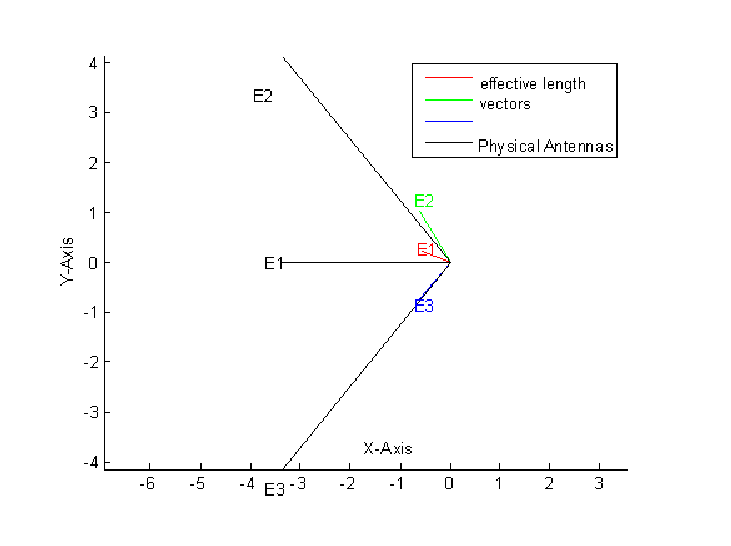
\includegraphics[width=1.0\linewidth]{paperpics/fig(2).eps}
\caption{Comparison of geometric and electric antennas} \label{fig:comparison}
\end{figure}



The effective length vectors often deviate considerably from the geometric antennas. Figure \ref{fig:comparison} shows the geometric antennas of the STEREO spacecraft in black, while the electric antennas are shown in color. For this calculation a frequency of 300kHz was used which is well within the quasistatic range. At high frequencies, where the wavelength of the incident wave is not large in comparison to the spacecraft dimensions, the effective lengths vector depends on frequency and direction of the radiation  (see eq. \ref{heff}) and its imaginary part becomes significant. Special care has to be taken when the effective length vectors are used in this range. Similar consideration has to be made in the case of SOLAR ORBITER.


\section{Quasi-thermal noise spectroscopy}
Quasi-thermal noise spectroscopy (QTNS) is a technique for finding the basic parameters of plasma by analyzing the electrostatic field spectrum measured by antennas. When the plasma frequency is higher than the cyclotron frequency, thermal motion excites Langmuir waves which are dependent of the velocity distribution function. The spectrum is cut off at the plasma frequency and has a peak just above. The cutoff bears information about the plasma density, the spectrum level about the temperature. The shape of the peak reveals information about the supra thermal electrons. Figure \ref{fig:qtn} shows an example and also one of the problems with thermal noise. Its intensity is normally higher than the intensity of many received radio emissions (a Type II burst in this example).

\begin{figure}
\centering
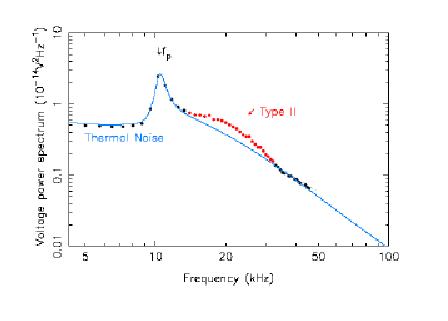
\includegraphics[width=1.0\linewidth]{paperpics/qtn.eps}
\caption{Example of quasi-thermal noise adapted after BEPI COLOMBO PWI Scientific and Technical Plan/Annex 2} \label{fig:qtn}
\end{figure}


\begin{figure}
\centering
\includegraphics[width=1.0\linewidth]{paperpics/debye.eps}
\caption{Variation of the Debye length as function of distance from the Sun} \label{fig:debye}
\end{figure}

One of the requirements necessary for QTNS works is that the length of the antennas must be at least of the order of magnitude of the Debye length. The spacecraft will operate at a distance from the sun of 0.2-0.9AU which corresponds to a Debye length of 2.5-11.5 meters (see Figure \ref{fig:debye}). It must be understood that the effective length vectors have to fulfill this requirement, not the geometrical antennas. The theory of an ideal dipole shows that its effective length vector is half its physical length. Calibration of similar spacecraft like STEREO has shown that the effective length vectors can be substantially shorter than without considering the base capacitances. Hence we recommend that this shortening of the effective length vectors is taken into account when planning the exact length of the antennas.

\section{Antenna Impedances}
The antenna impedance is an important property to describe an antenna. It describes the way an antenna is seen as part of the circuit and it determines how much the base capacitances influence the reception behavior.
Figure \ref{fig:imps} shows the antenna impedance of the STEREO antennas as function of frequency.

\begin{figure}
\centering
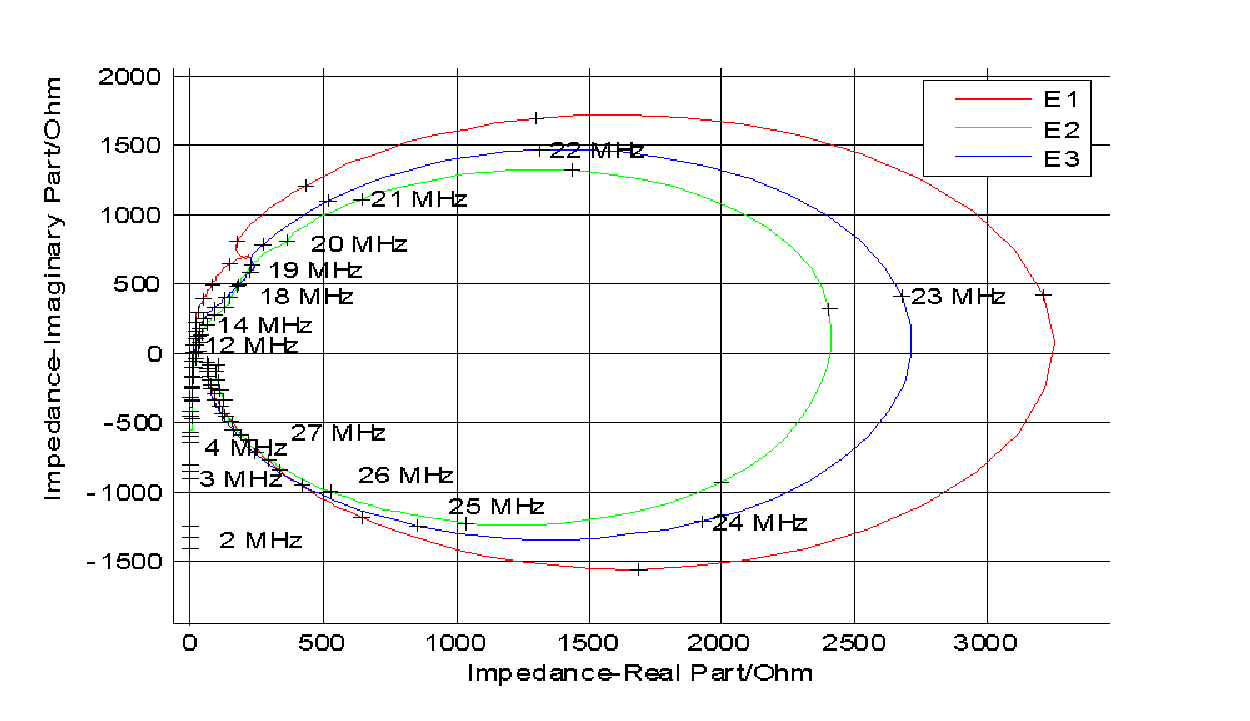
\includegraphics[width=1.0\linewidth]{paperpics/imps.eps}
\caption{Antenna Impedances of the SWAVES antennas. The imaginary part is plotted against the real part.} \label{fig:imps}
\end{figure}

\section{Conclusion}
SOLAR ORBITER is a very ambitious space mission currently in the planning phase. Onboard will be a radio experiment comprising either 3 or four antennas. Even though the final configuration is not yet determined, some properties and important points to be considered can be deduced on basis of the experience with former analysis of other spacecraft antennas.

In this paper we treated several aspects which will be important to consider when dealing with the monopole antennas of SOLAR ORBITER.



\section*{Acknowledgments}
These studies were supported by the Austrian Space Applications Programme (ASAP).



   \bibliographystyle{aa}
   \bibliography{../../Bibliography/MyBib}

\end{document}
%%
%% <<<<< End of generated file <<<<<<
%%
%% End of file `esapub.tex'.
